%________________________________________
%CaRS Move I "Establish a territory" (Situation):
% * Important area
% * Introducing and reviewing items of previous  research <--(ToDO)
Ship dynamics predictive models have a wide range of applications, e.g., safety enhancements, route planning and optimization, autonomous shipping, etc., \citep{aslam_internet_2020}.
Ship manoeuvring is a sub field of ship dynamics with well established system based models such as: \citet{abkowitz_ship_1964,nomoto_steering_1957,norrbin_theory_1971}, and the MMG model \citep{yasukawa_introduction_2015}.

Captive model test is the classical method to identify the parameters within these models. However, for the full scale ships, this method is not practically applicable, while computational fluid dynamics (CFD) with either direct simulations or virtual captive tests (VCT) has emerged as an interesting option \citep{liu_predictions_2018,li_ship_2022}.
The CFD requires a complete understanding of the system. Acquiring such knowledge may be possible for some simplified scenarios, but huge modelling uncertainties are expected when applied in a complex sea environment including wind, wave and current \citep{miller_ship_2021}. 
Even if the sea is flawlessly modelled, long-term predictions with high accuracy will be exposed to deterministic chaos \citep{lorenz_deterministic_1963}.
Together with the other drawbacks of CFD -- such as high computational costs -- data driven models have become an attractive alternative or complement, with an increased number of publications in the past 10-15 years (shown in Fig.\ref{fig:pub_overview}) -- especially within the field of autonomous ships \citep{ahmed_survey_2023}.
%
\begin{figure}[h]
  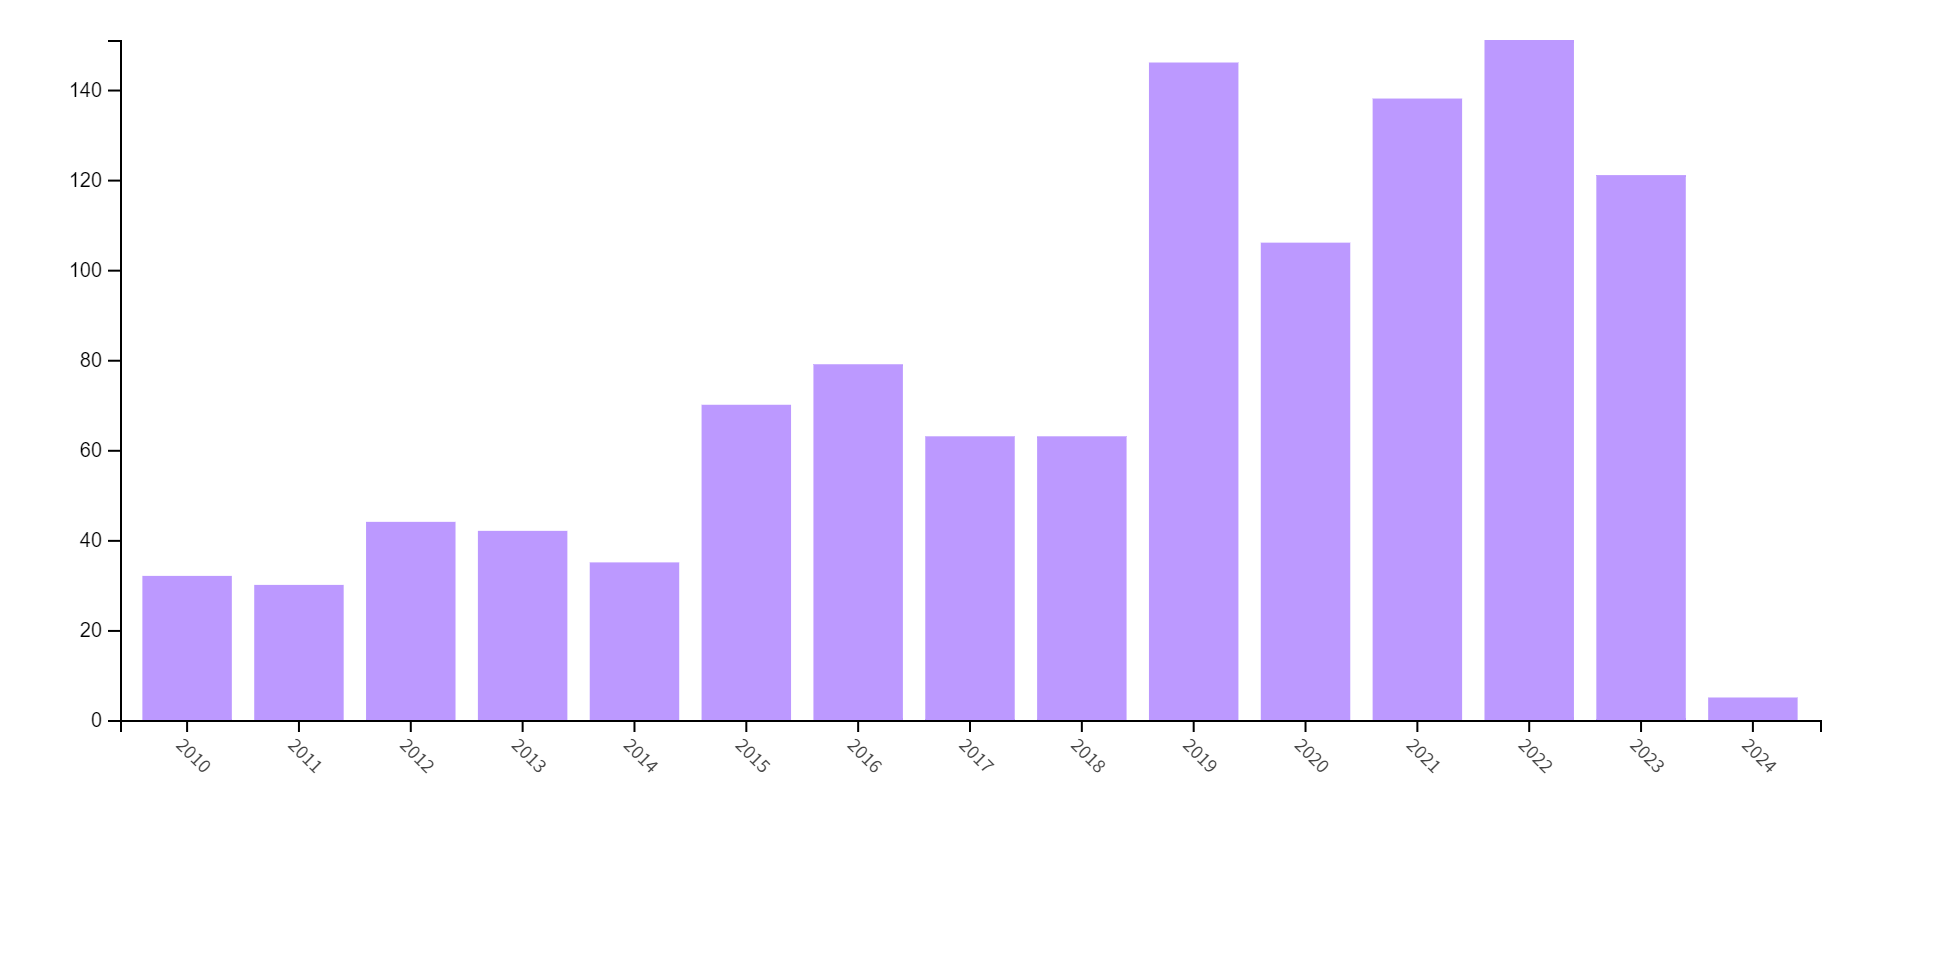
\includegraphics[width=.5\textwidth]{figures/trendinyear.jpg}
  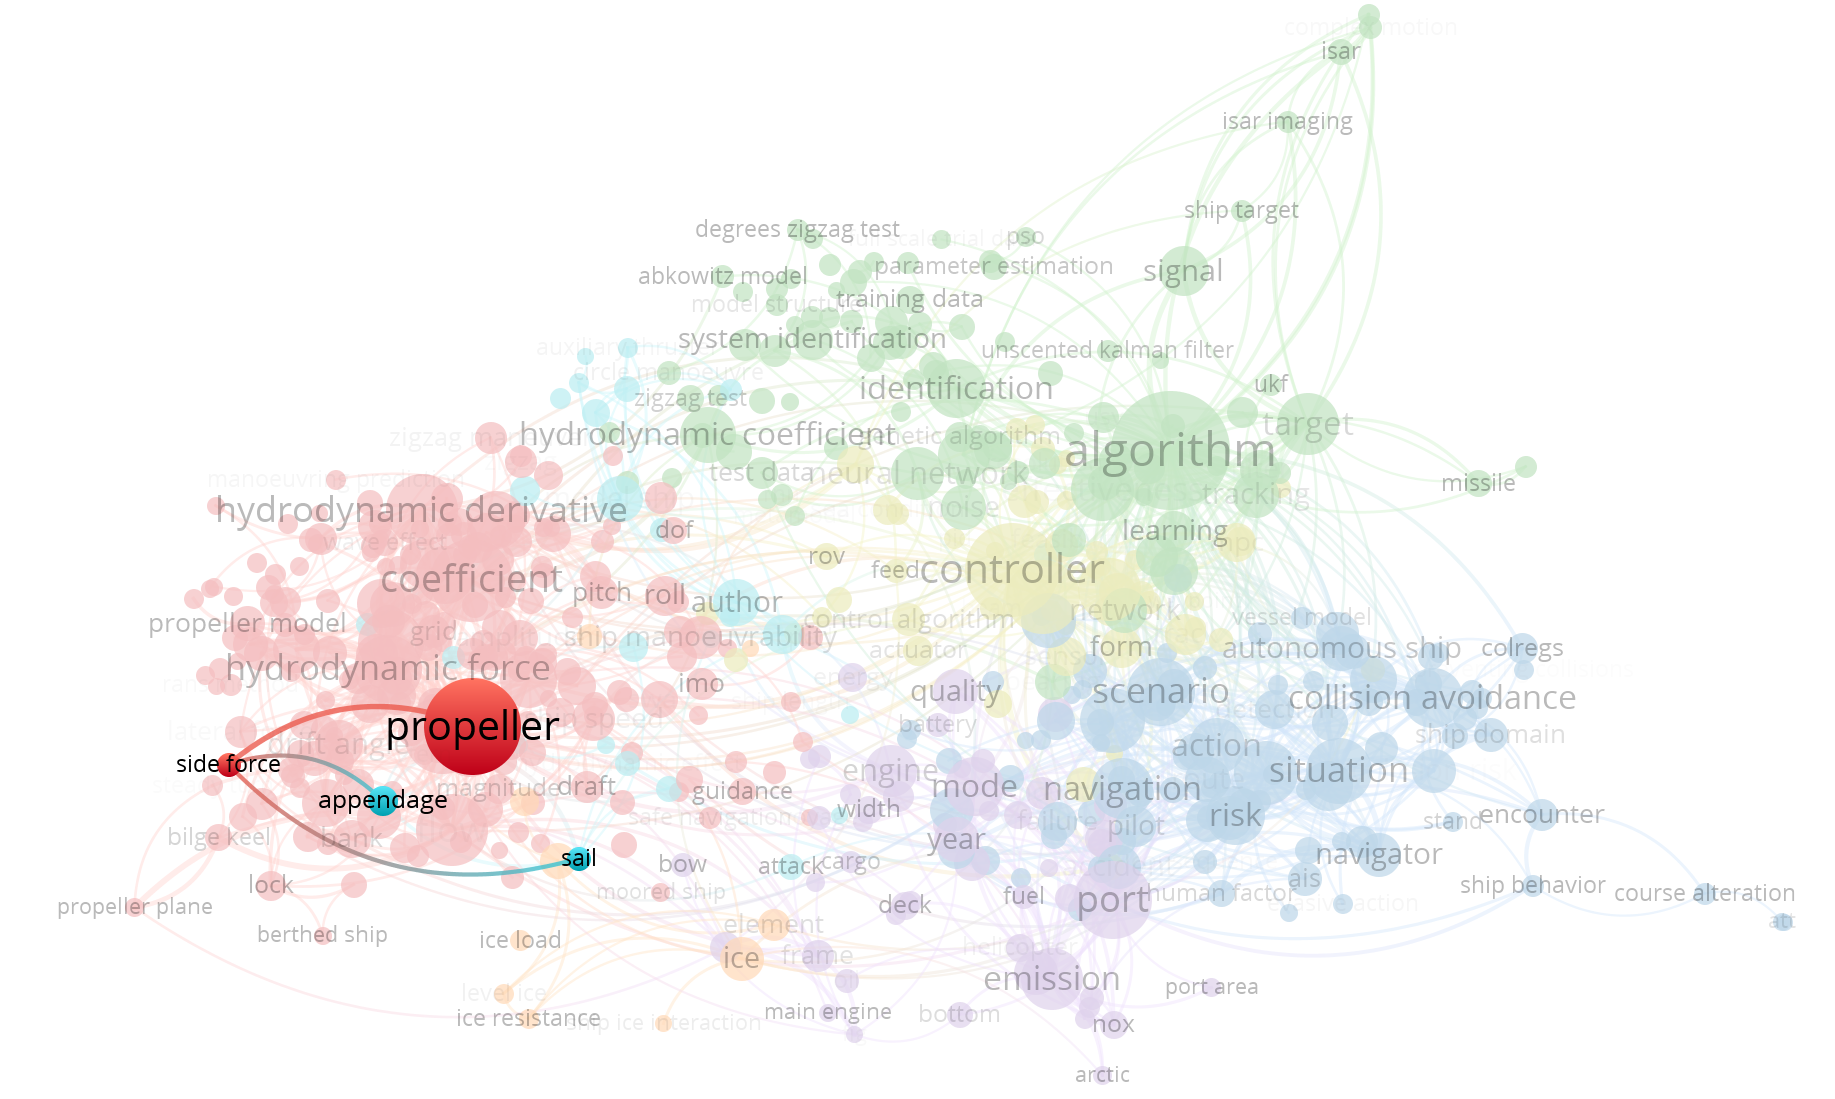
\includegraphics[width=.5\textwidth]{figures/wind_drift_research.png}
  \caption{Research topics within the field of ship maneuverability system identification}
  \label{fig:pub_overview}
\end{figure}
%

Many of these papers have shown that hydrodynamic coefficients can effectively be estimated on simulated data where the exact ''physical'' model is assumed known. However, in real cases/applications, the mathematical model is just the simplification of real physics (from VCT, model test, sea trials, or full-scale tests), while the complexity of hydrodynamics involved in vessel maneuvering will greatly challenge the simplified empirical mathematical methods without carefully considering the actual physics inside hydrodynamic coefficients and their interactions. 

One of the earlier papers with real data was proposed in 1976 by \citet{astrom_identification_1976} to develop a linear manoeuvring model that utilized manually recorded data in 1969 aboard the Atlantic Song freighter with Kalman filter (KF) and maximum likelihood estimation. 
The extended Kalman filter (EKF) was used on a nonlinear Nomoto model by \citet{perera_system_2015}, a 3 degree of freedom model by \citet{shi_identification_2009}, and a recursive EKF by \citet{alexandersson_system_2022}.
The unscented Kalman filter (UKF), which has been proposed as an improvement to the EKF for handling nonlinear systems, was used in \citet{revestido_herrero_two-step_2012}.
Support vector regression (SVR) has been investigated by \citet{luo_parameter_2016}, \citet{zhu_parameter_2017}, and \citet{wang_parameter_2021}. 

%
%________________________________________
%CaRS Move II "Establish a niche" (Problem):
% * counter claim?
% * gap?
% * question       <------
% * continuation?
The regressors of the data-driven ship manoeuvring models are often strongly linearly dependent. This multicollinearity is a well known issue in parameter identification, that may lead to parameter drift and poor generalization. The parameters are thus mathematically correct but physically incorrect \citep{luo_parameter_2016}. 
An example of generalization is when a model identified on calm water data is exposed to wind, where a drift angle is now needed to maintain a straight course. This wind state is rare in calm water manoeuvring tests, where the drift angle is almost exclusively accompanied by yaw rate (see \autoref{fig:phase_portrait}); 
The regression will thus have problems to distinguish between these quantities.
% Wengang fixes a better figure here...
%This drifting (side forces) is rarely investigated as shown in %\autoref{fig:pub_overview}.
%
\begin{figure}[h]
  \centering
  \includesvg{figures/multicollineraity.multicollinearity.svg}
  \caption{Phase portrait where the combination of drift angle and yaw rate is shown for zigzag10/10, and zigzag20/20 tests.}
  \label{fig:phase_portrait}
\end{figure}
Using more informative data or simplifying the model -- when possible -- and thereby reducing the number of parameters, is one of the most researched ways to mitigate the multicollinearity. Other possible remedies are the difference method \citep{luo_parameter_2016}, principal component analysis (PCA), and partial least squares regression \citep{jian-chuan_parametric_2015}. 
%________________________________________
%CaRS Move III "Occupy the niche" (Solution/Evaluation):
% * outline purpose?                        <--
% * list research questions?                <--
% * announce principal findings?            
% * stating the value of present research?
% * article structure?                      <--

More remedies are however needed; Therefore, in this paper, a physics informed manoeuvring model (PISM), which features a new semi-empirical rudder model based on semi-empirical formulas from the literature, is proposed.

The objective is to identify a model that is not just mathematical correct, but also as physically correct as possible.
To evaluate the physical correctness, two unique datasets from a wind-powered pure car carrier (wPCC) are employed following a research workflow as summarized in \autoref{fig:methodology}.
Data from VCT at various steady-state drift angles, yaw rates, and rudder angles, establish the physically correct kinetics in an identified reference model. 
System identification is conducted via inverse dynamics \citep{faber_inverse_2018} on a second dataset containing a series of manoeuvring model tests with a free model of the WPCC. The identification is conducted for the PISM as well as an mathematical manoeuvring model. The identifications are compared to the reference model and the generalization of the models is also studied in an idealized wind state.
%
\begin{figure}[h]
  \centering
  %\includesvg[width=\columnwidth, pretex=\scriptsize, height=12cm]{figures/methodology2.svg}
  \includesvg[pretex=\centering\fontsize{7.5}{8}]{figures/methodology2.svg}
  \caption{Research workflow.}
  \label{fig:methodology}
\end{figure}

The left of the paper is organized as follows. The proposed physics informed manoeuvring model is first presented in \autoref{sec:ship_models}, while some mathematical details of the model are given in the appendix. 
The developed methodology framework to identify parameters within the PISM is described in \autoref{sec:methodology} -- including the VCT regression, and the inverse dynamics. The case study ship with wind propulsions is briefly described in \autoref{sec:case_study}, as well as some known parameters of the ship's manoeuvring model. Results are presented in \autoref{sec:results}, followed by some key conclusions of this research in \autoref{sec:conclusions}.